\documentclass[12pt]{article}

 %%%
 \usepackage[utf8]{inputenc}
 \usepackage{graphicx}
 \usepackage{xcolor}
 \usepackage{hyperref}
 \hypersetup{colorlinks, linkcolor = black, citecolor = black, filecolor = black, urlcolor = [RGB]{227, 114, 34}}
 \usepackage{float}
 \usepackage{geometry}\geometry{a4paper, total={170mm,257mm}, left=20mm, top=20mm}

 \definecolor{PIKorange}{RGB}{227, 114, 34}
 \definecolor{PIKgray}{RGB}{142, 144, 143}

 \title{ \bfseries \color{PIKorange} Japan: information on national emissions, population and GDP, and mitigation targets}

 %%%

 \begin{document}

 \maketitle

 %%%
 \noindent \textbf{Authors:} \newline
 \indent Annika Guenther$^{1}$ \newline
 \indent Johannes Guetschow$^{1}$ \newline
 \noindent \textbf{Affiliations:} \newline
 \indent 1. Potsdam Institute for Climate Impact Research, Germany \newline
 \noindent \textbf{DOI:} [to be added] \newline

 \textbf{TODO}
 \begin{itemize}
 \item Table with info on target (main and reclass; emissions from NDC; target quantis + plot).
 \item GWP: NDC emissions coverted from AR2 to AR4 by national conversion factor (2010--2017, PRIMAP-hist v2.1).
 \item References!
 \end{itemize}

 \newpage %%%
 \section{Non-LULUCF emissions and socio-economic data}
 \label{sec:nonLULUCFSocioEco}
 With national emissions of 1.3~Gt CO$_2$eq, Japan contributed 2.7\% to global emissions in 2017, while in 2030 its share is estimated to decrease to 2.2\% (Table~\ref{tab:overview}).
 The estimates for 2030 are based on the downscaled SSP2 Middle of the Road marker scenario (dmSSP2), in which Japan is estimated to emit 1.2~Gt CO$_2$eq in 2030.
 That change in emissions would constitute a decrease of -5.6\% compared to 2017. 
 The pathways dmSSP1--5 show a range of 1.1--1.5~Gt CO$_2$eq in 2030, and 0.9--2.0~Gt CO$_2$eq in 2050.
 The country's global rank in terms of total emissions per unit of GDP was 162 in 2017, and 40 regarding the per-capita emissions (149 and 42 in 2030).
 In terms of accumulated historical emissions, Japan contributed to the global 1850--2017 emissions by 3.1\%. 
 When only accounting for the years 1990--2017, its contribution increases to 3.5\%.
 All of the emissions are presented following GWP~AR4, and exclude emissions from LULUCF (exclLU), and bunkers fuels emissions (exclBunkers).

 \begin{table}[H]
 \centering
 \caption{National emissions (dmSSP2), GDP and population for Japan, together with the emissions per unit of GDP and per capita emissions (all for 2017 and 2030). 
 Additionally, the global share and its rank are displayed.}
 \label{tab:overview}
 \begin{tabular}{l || l r l r r}
 \bfseries  & \bfseries Year & \bfseries Total & \bfseries Unit & \bfseries Glob. share & \bfseries Rank \tabularnewline \hline \hline
 \bfseries Emissions & 2017 & 1.3 & Gt CO$_2$eq & 2.7\% & 5 \tabularnewline 
 \bfseries  & 2030 & 1.2 & Gt CO$_2$eq & 2.2\% & 7 \tabularnewline \hline
 \bfseries GDP & 2017 & 5.1 & Trillion 2011~GK\$ & 4.5\% & 4 \tabularnewline 
 \bfseries  & 2030 & 5.6 & Trillion 2011~GK\$ & 3.1\% & 5 \tabularnewline \hline
 \bfseries Emissions & 2017 & 255.6 & t CO$_2$eq / Million 2011~GK\$ & 0.2\% & 162 \tabularnewline 
 \bfseries per GDP & 2030 & 216.3 & t CO$_2$eq / Million 2011~GK\$ & 0.2\% & 149 \tabularnewline \hline
 \bfseries Population & 2017 & 127.5 & Million Pers & 1.7\% & 10 \tabularnewline 
 \bfseries  & 2030 & 122.4 & Million Pers & 1.5\% & 13 \tabularnewline \hline
 \bfseries Emissions & 2017 & 10.1 & t CO$_2$eq /  Pers & 0.7\% & 40 \tabularnewline 
 \bfseries per capita & 2030 & 10.0 & t CO$_2$eq /  Pers & 0.7\% & 42 \tabularnewline 
 \end{tabular}
 \end{table}

 For Japan, in 2017 the main emissions share on sectoral level (Fig.~\ref{fig:tsEmi}) came from the Energy sector (87.9\%), followed by IPPU (7.8\%)
 The Kyoto~GHG with the highest emissions in 2017 was CO$_2$, constituting as much as 91.9\% of the national emissions. 
 Second largest contributor was HFCs (3.5\%)
 The total of F-gasesonly represented 3.9\%.
 The total CO$_2$ emissions are expected to be 88.6\% of the national Kyoto~GHG emissions in 2030 (dmSSP2).

 \begin{figure}[H]
 \centering
 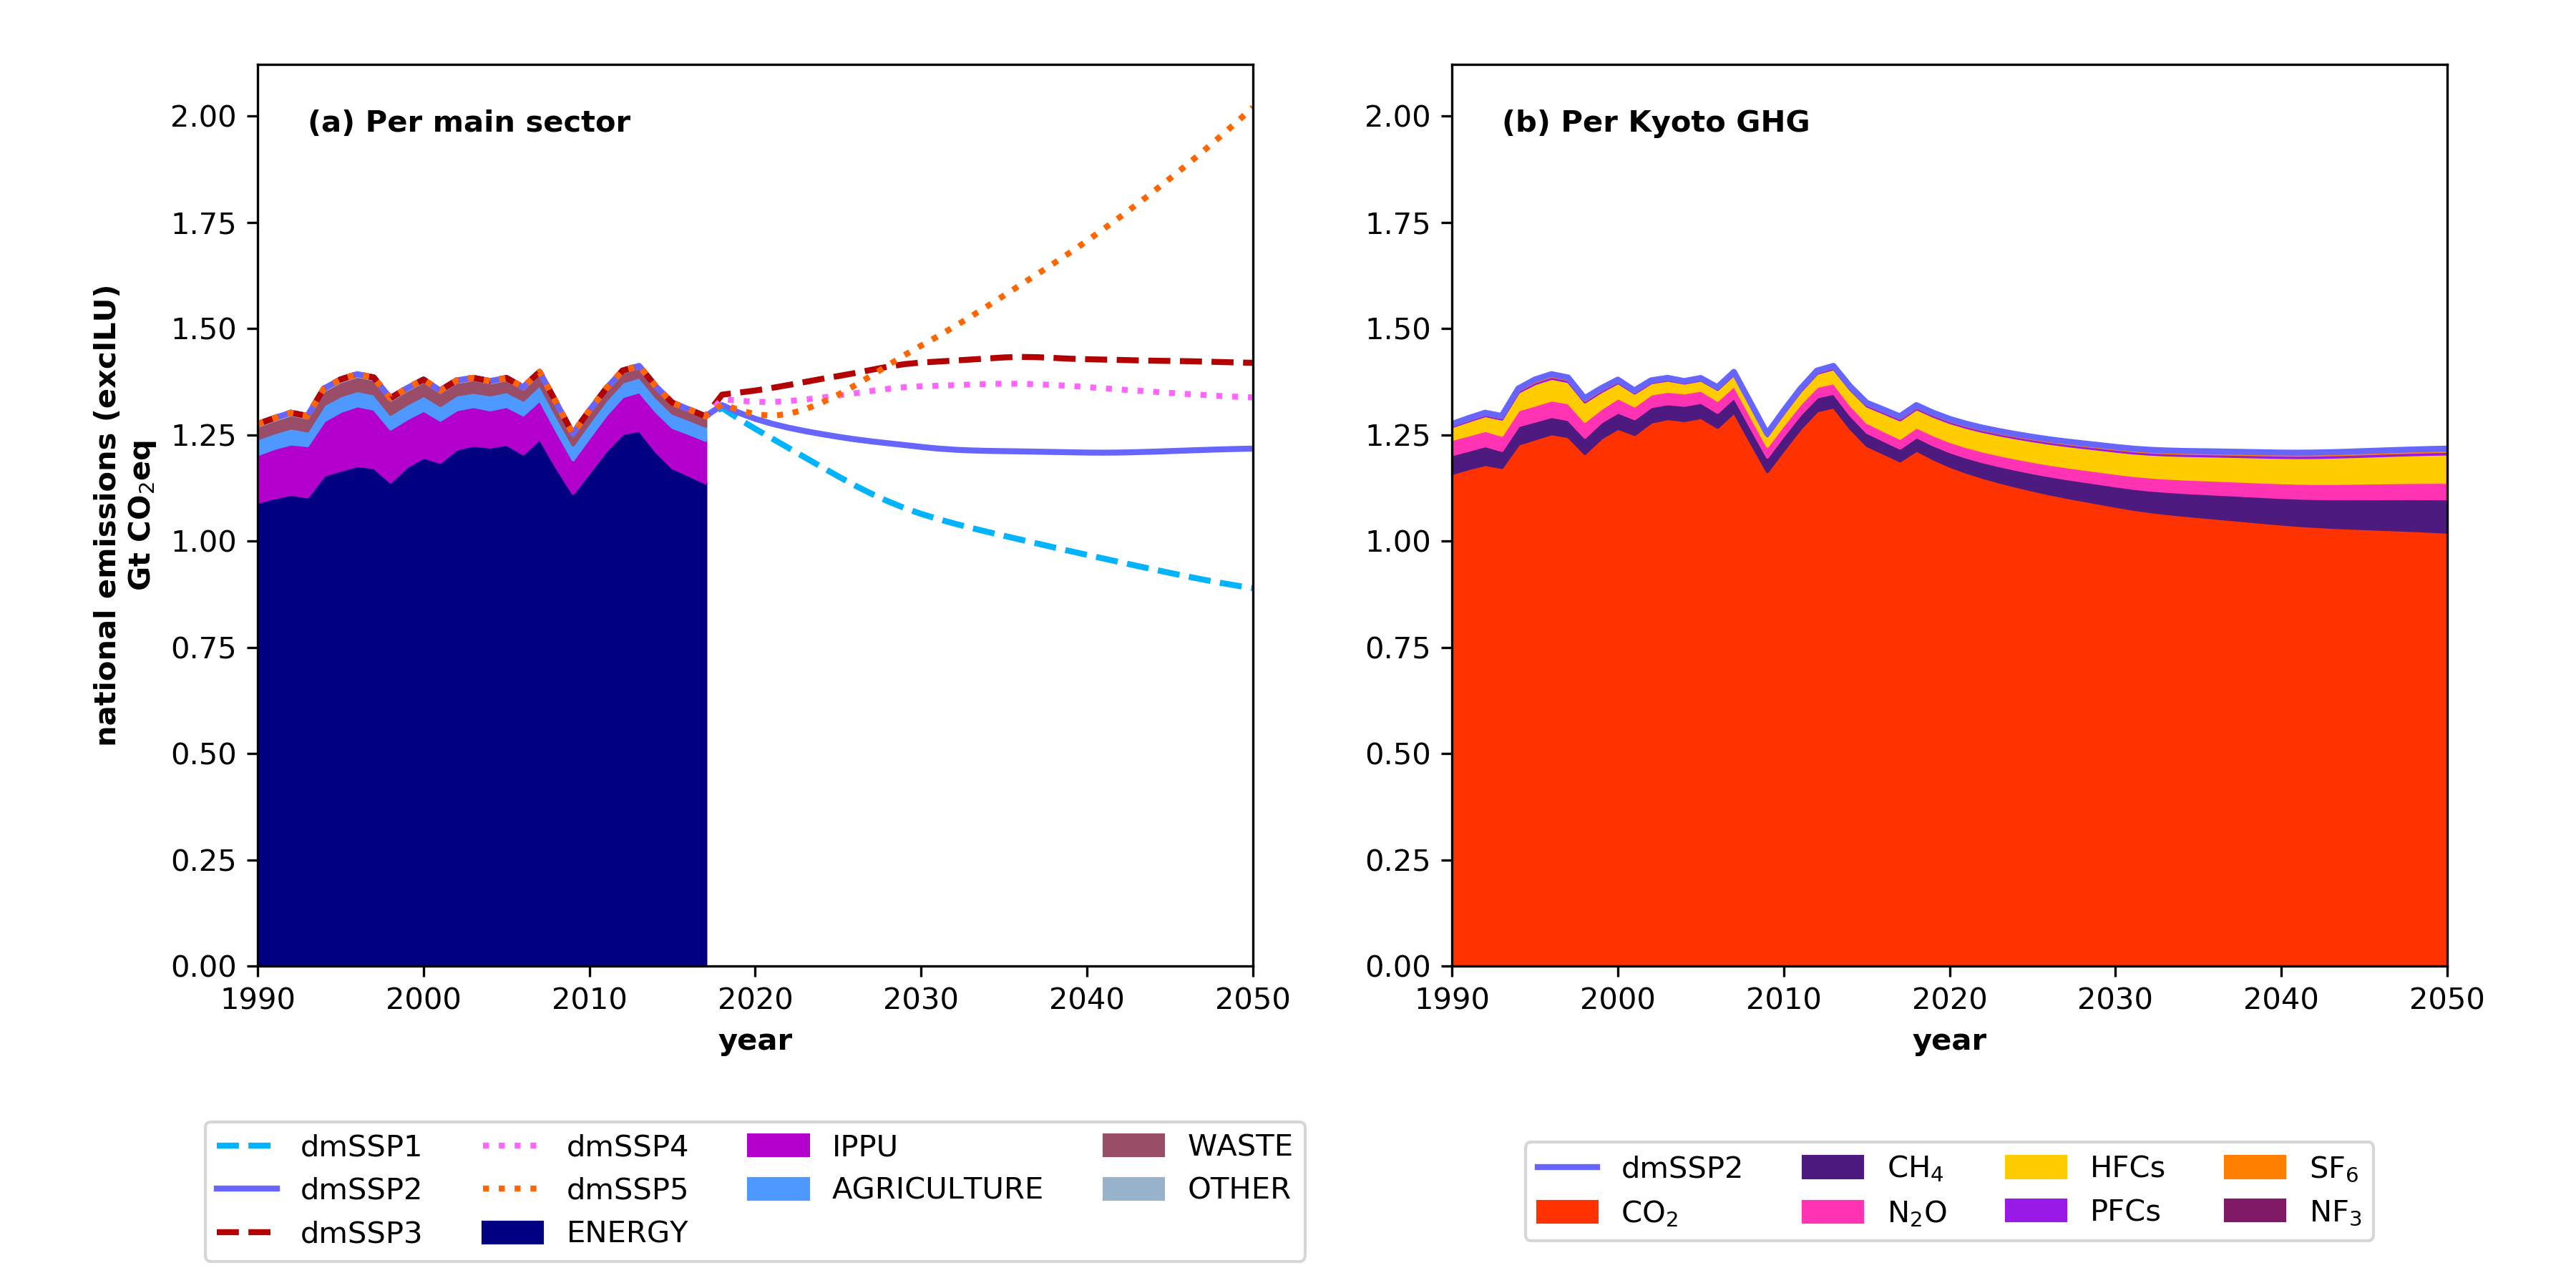
\includegraphics[width=\textwidth]{C:/Users/annikag/primap/ndc_quantifications/latex_files/JPN/ts_emi_exclLU_JPN.png}
 \caption{'Stacked' timeseries of national emissions (exclLU) per main-sector (a) and Kyoto~GHG (b). 
 No information available on the sectoral contributions after 2017.}
 \label{fig:tsEmi}
 \end{figure}

 \begin{figure}[H]
 \centering
 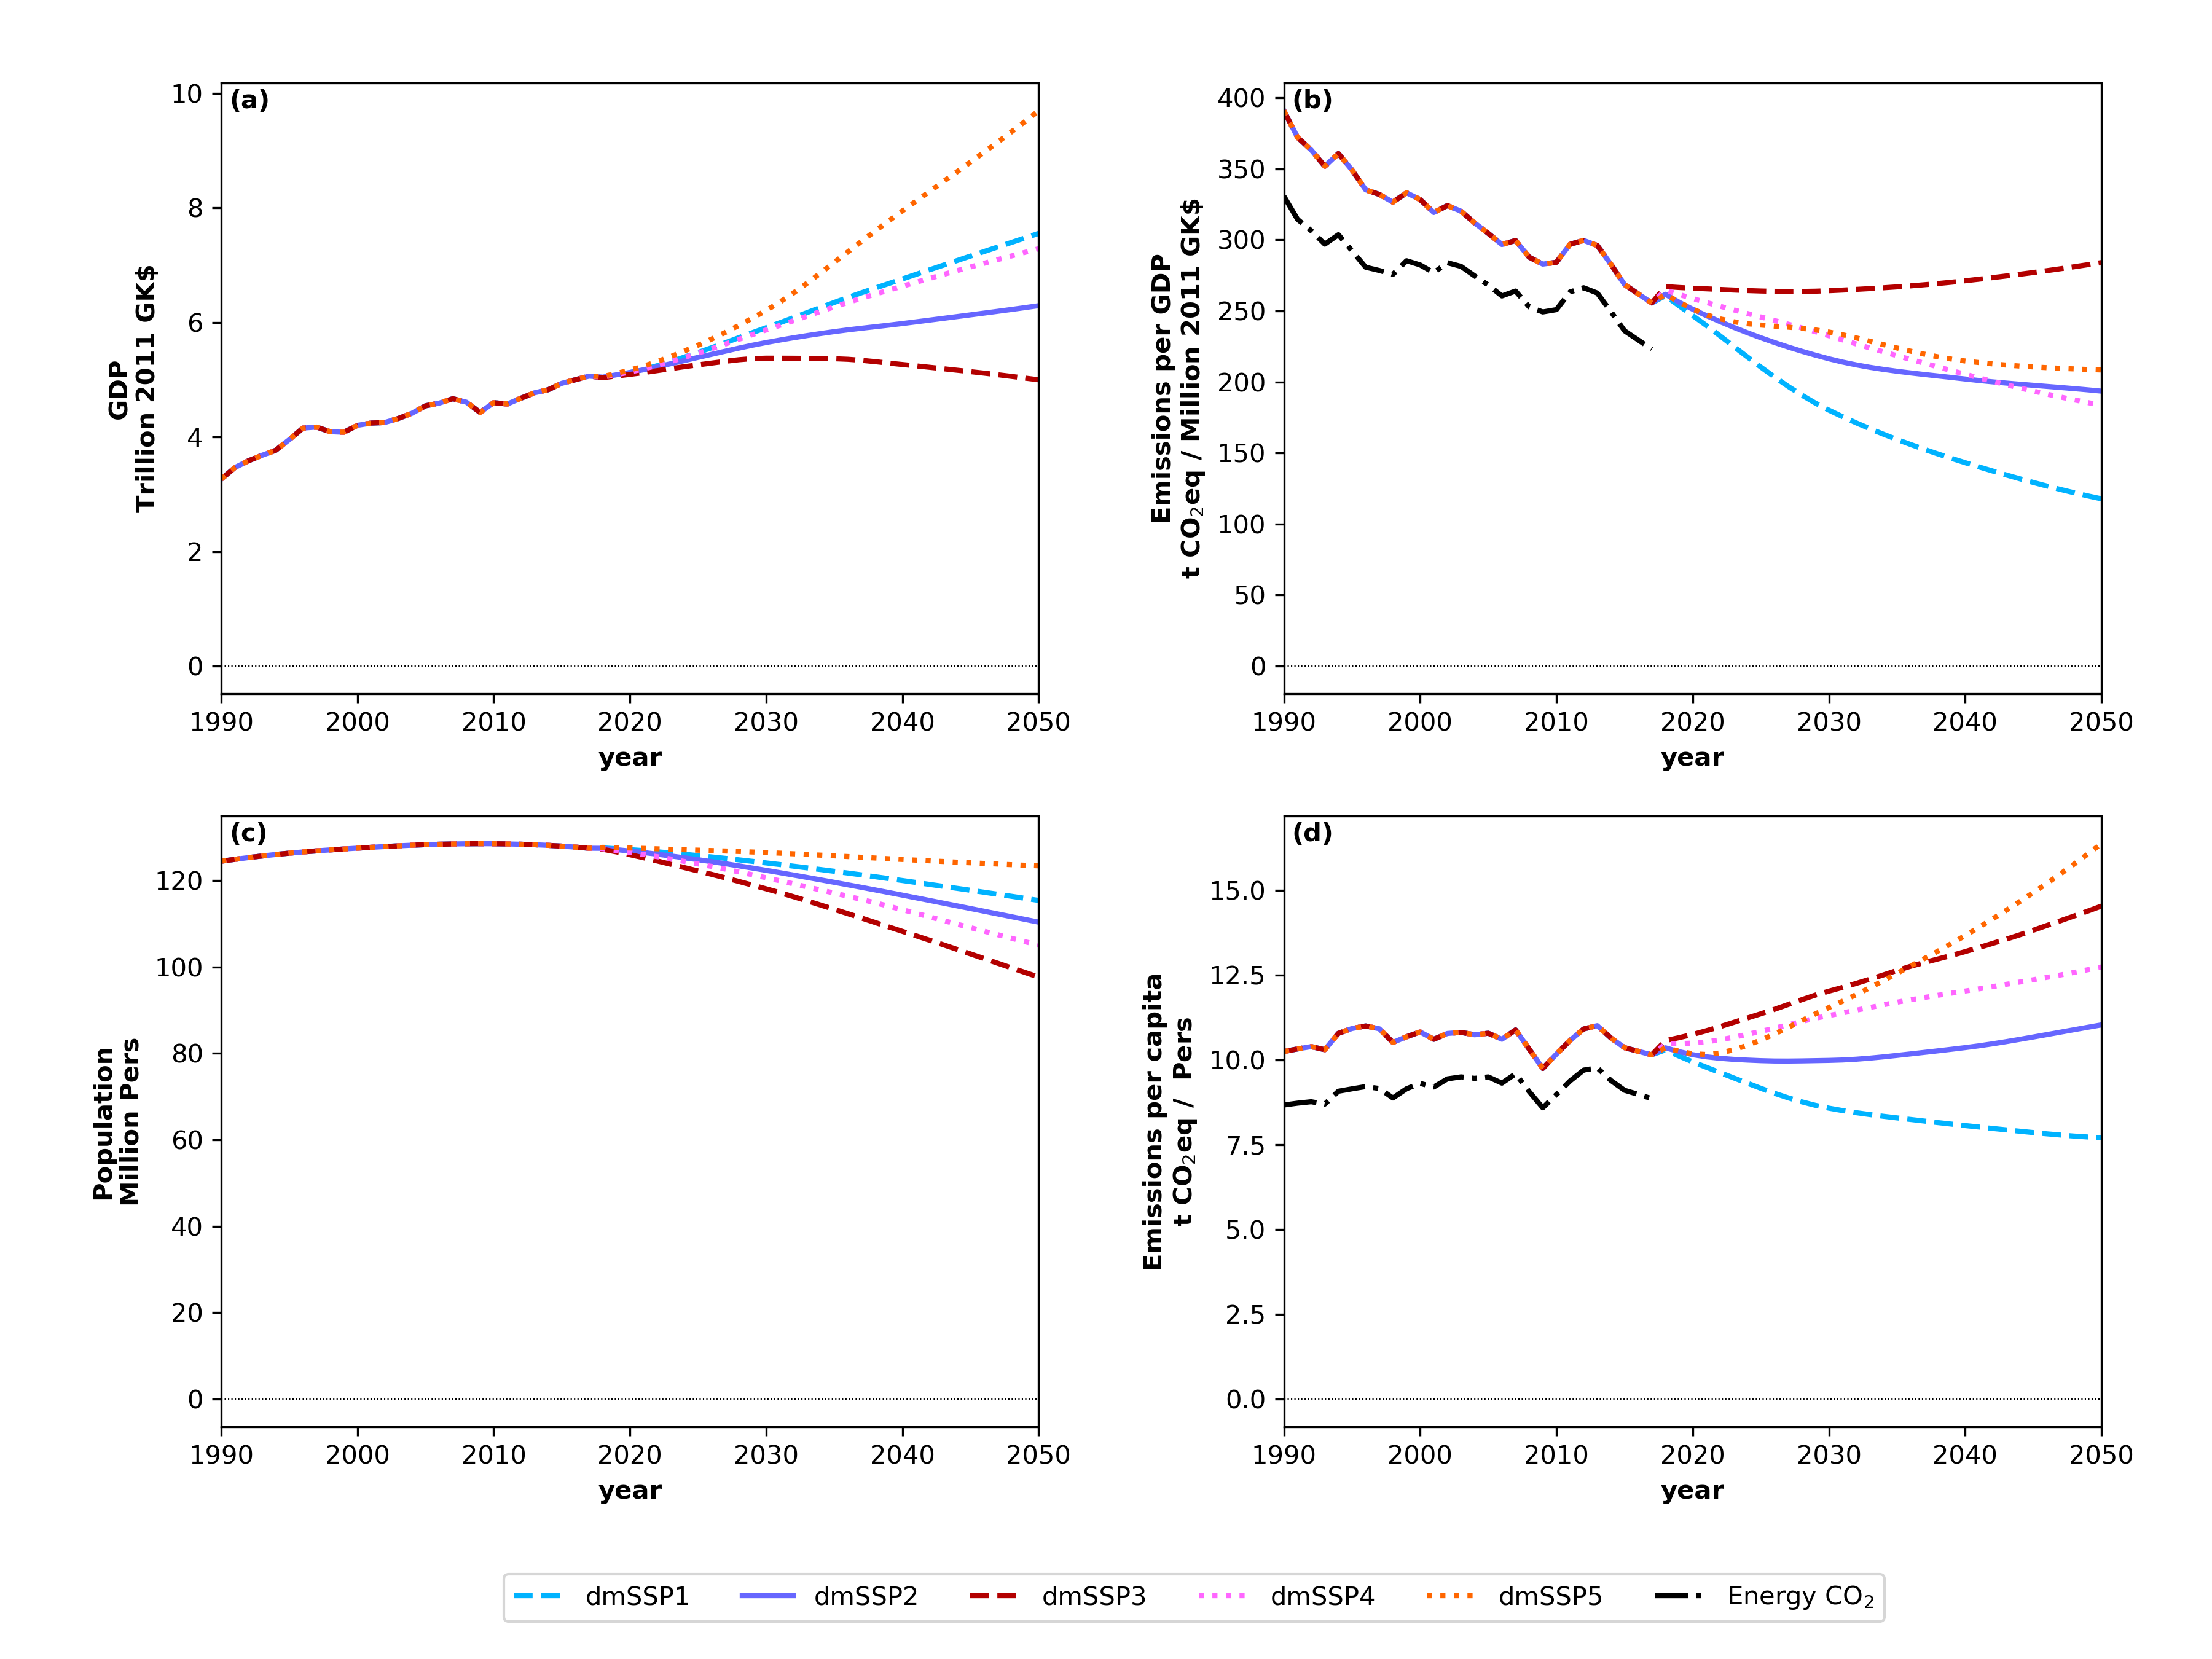
\includegraphics[width=\textwidth]{C:/Users/annikag/primap/ndc_quantifications/latex_files/JPN/ts_gdp_pop_JPN.png}
 \caption{Timeseries of national GDP (a) and population (c), and Kyoto~GHG emissions (exclLU, exclBunkers) per unit of GDP (b) or per capita (d).}
 \label{fig:tsSocioEco}
 \end{figure}

 The national GDP increased in recent years, and the emissions per unit of GDP had an opposite trend (Fig.~\ref{fig:tsSocioEco}).
 The population decreased, while the per capita emissions dropped. 
 Following dmSSP2, the GDP is projected to increase towards 2050. 
 The emissions per GDP are estimated to rise after 2017 but to decrease again before 2050. 
 Japan's population is assumed to diminish towars 2050, and the per capita emissions are expected to increase towards 2050. 

 \newpage %%%
 \section{LULUCF emissions}
 \label{sec:emiLULUCF}
 LULUCF emissions data for Japan are available from the following sources (Fig.~\ref{fig:tsLULUCF}): CRF (2019), CRF (2018), FAO (2019).

 \textbf{High fluctuations? Data gaps? Difference between sources?}

 \begin{figure}[H]
 \centering
 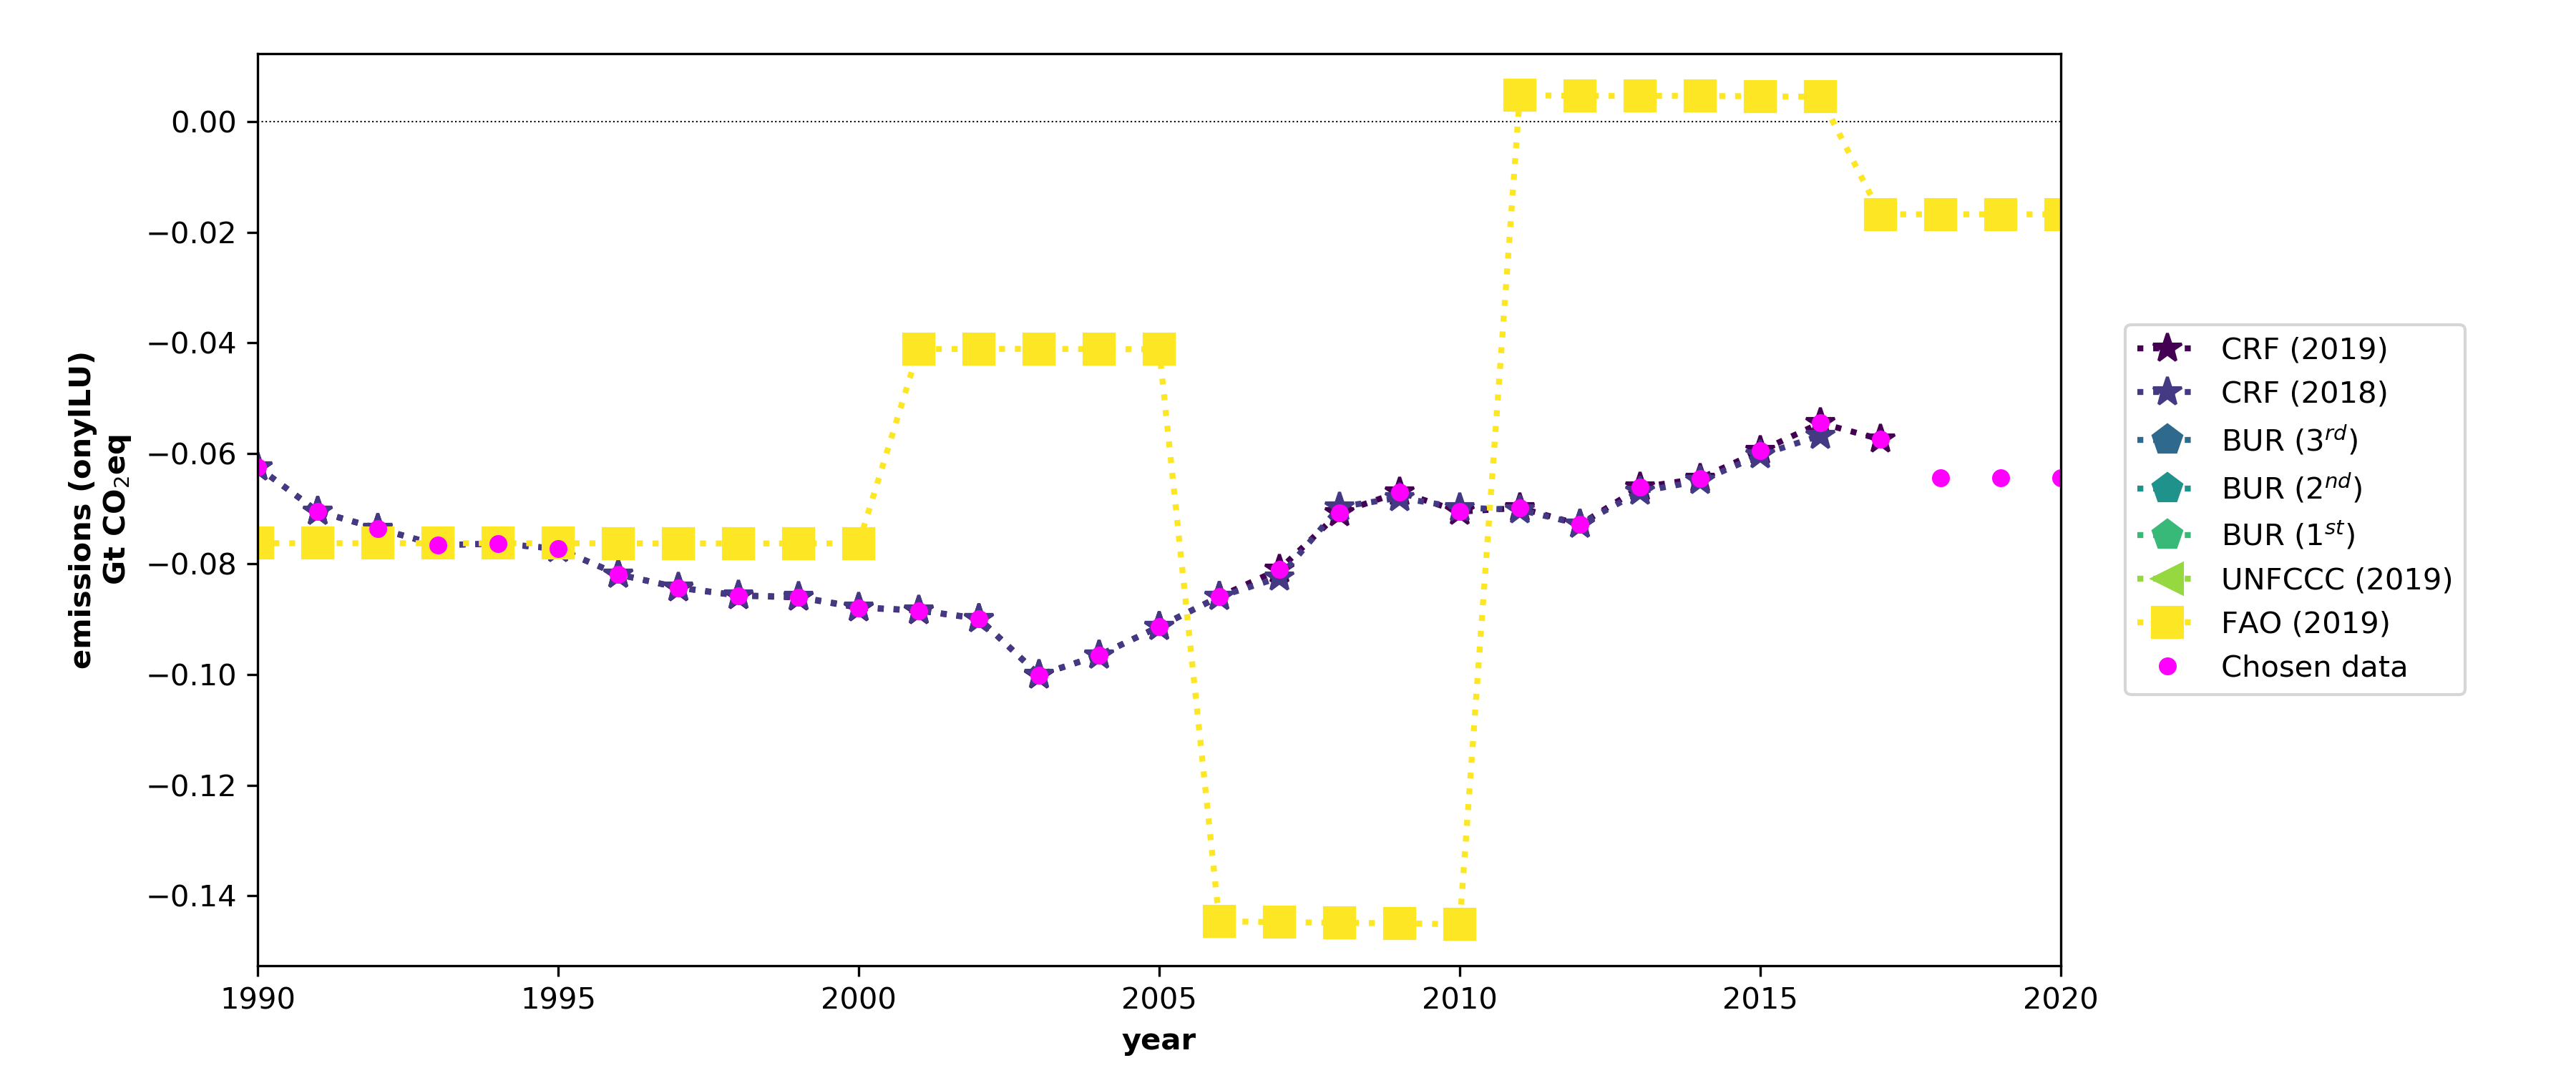
\includegraphics[width=\textwidth]{C:/Users/annikag/primap/ndc_quantifications/latex_files/JPN/ts_emi_onlyLU_JPN.png}
 \caption{Timeseries of emissions from LULUCF (CO$_2$ plus CH$_4$ and N$_2$O) as available from different data-sources. 
 Indicated in pink are the 'chosen' data, as used in our assessment of Japan's NDC (if needed). 
 The pink timeseries was inter- and~/ or extrapolated (interpolation: linear, extrapolation: constant).}
 \label{fig:tsLULUCF}
 \end{figure}

 \newpage %%%
 \section{Mitigation targets (NDC)}
 \label{sec:mitiTars}

 \textbf{ 
 Give the \%cov for the base and target year (and 2017).
 Global share for 2030 for the mitigated pathways and \% reduction relative to 1990 and 2017.
 Table with the 'input' data and the resulting targets (like ndcs\_targets.csv).}
 Japan has an NDC, with a GHG mitigation target of the type RBY (base year target; main target type).
 The reclassified target type is ABS (absolute emissions target).

 \begin{table}[H]
 \centering
 \caption{Information on Japan's GHG mitigation target(s).}
 \label{tab:mitiTars}
 \begin{tabular}{l l l l l l l }
 \bfseries type & \bfseries condi. & \bfseries range & \bfseries value & \bfseries refYr & \bfseries tarYr & \bfseries LU \tabularnewline \hline
 RBY & uncondi. & best & -26\% & 2013 & 2030 & inclLU \tabularnewline 
 ABS & uncondi. & best & 1042 Mt~CO$_2$eq AR4 & 2013 & 2030 & inclLU \tabularnewline 
 ABS & uncondi. & best & 1079.40 Mt~CO$_2$eq AR4 & 2013 & 2030 & exclLU \tabularnewline 
 \end{tabular}
 \end{table}

 \begin{figure}[H]
 \centering
 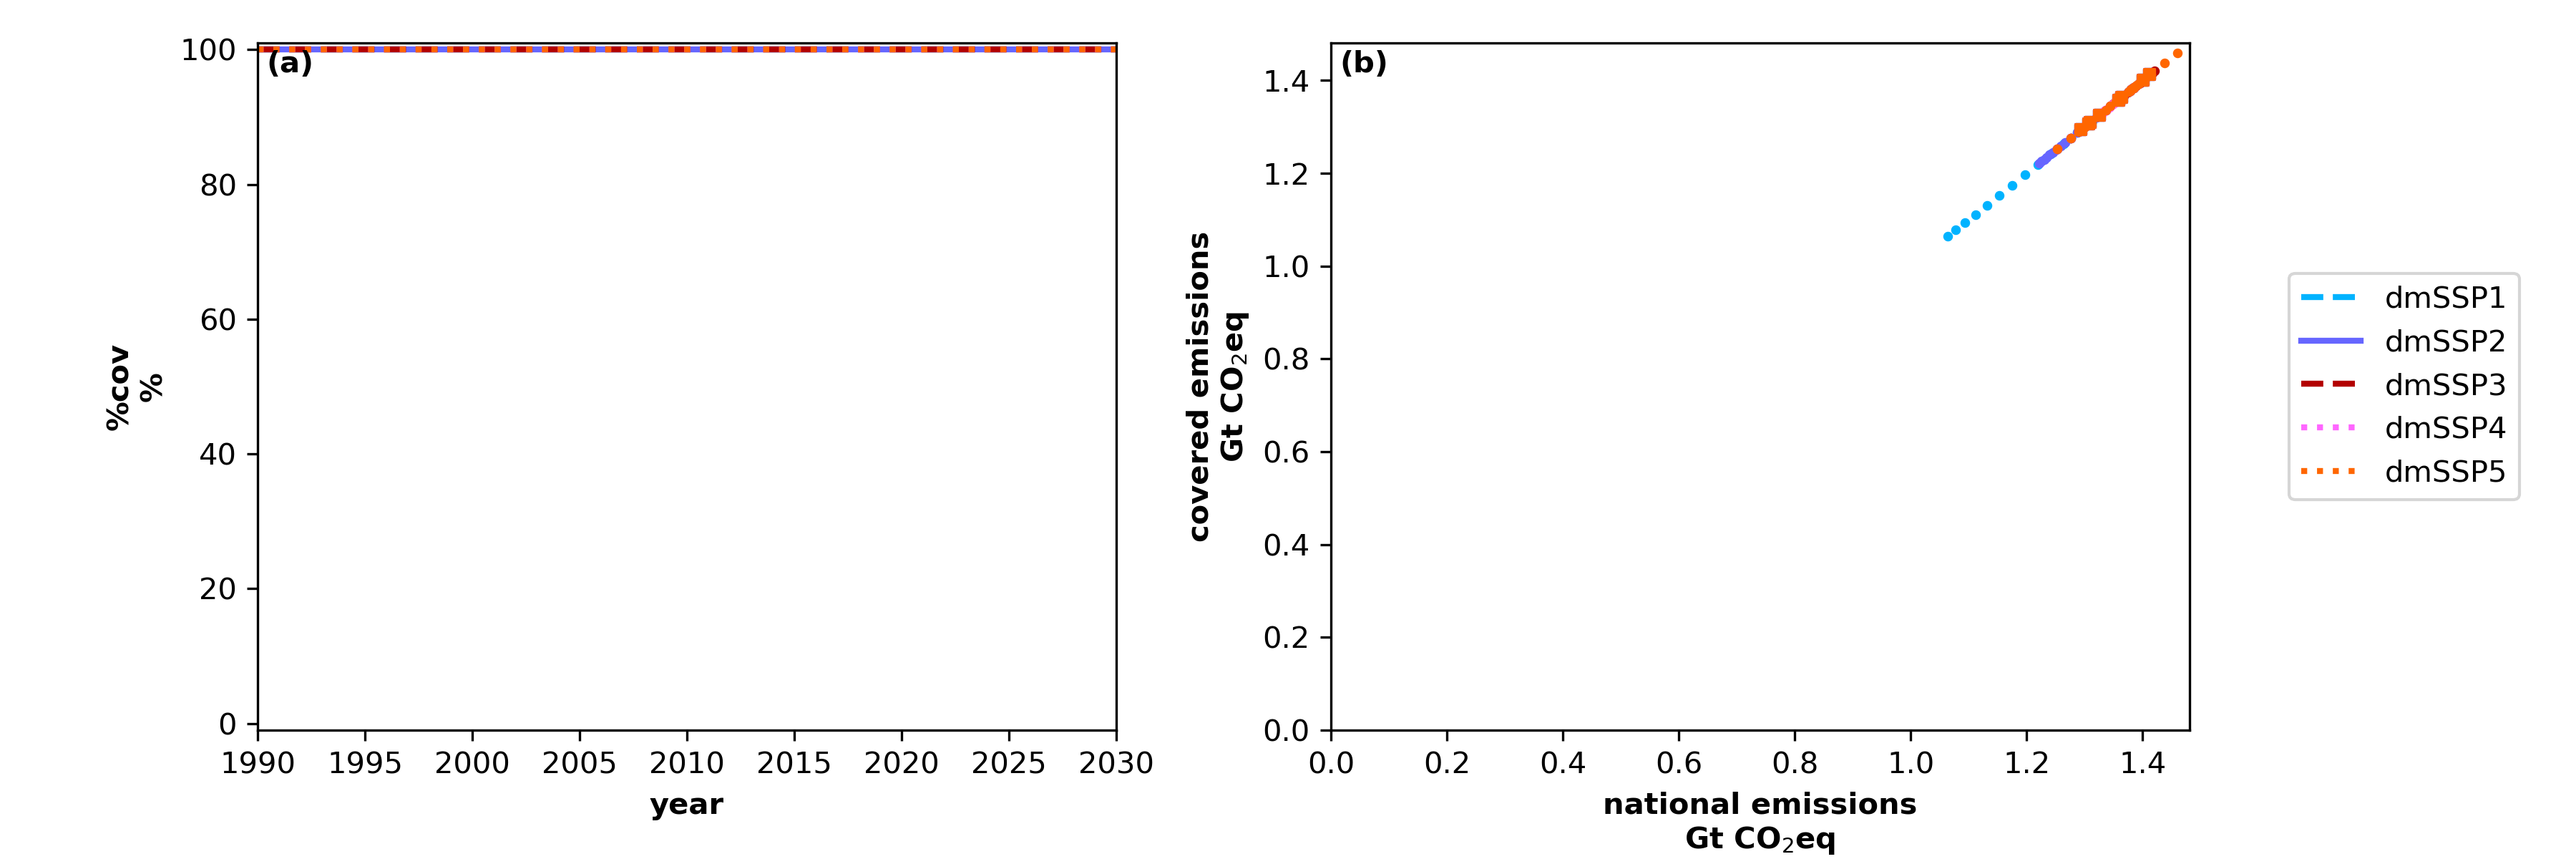
\includegraphics[width=\textwidth]{C:/Users/annikag/primap/ndc_quantifications/latex_files/JPN/ts_pc_cov_JPN.png}
 \caption{Timeseries of Japan's national emissions (exclLU) and the share of emissions that is assumed to be covered by Japan's mitigation target.}
 \label{fig:tsPcCov}
 \end{figure}

 \begin{table}[H]\small
 \centering
 \caption{Information on covered sectors and gases as retrieved from NDC and adapted ('Adap.': used to calculate \%cov), and their shares in Japan's 2017 emissions (exclLU, exclBunkers; total 1.3~Gt CO$_2$eq).
 If either the sector or gas is assessed as 'not-covered', the emissions from this sector-gas combination are counted as not-covered (--). 
 Else the emissions are counted as covered (+; covered shares given in bold).
 (/) means that no information is available.
 LULUCF: NDC '+' and adapted '+' (estimated as a net sink of -0.1~Gt CO$_2$eq in 2017; based on the 'chosen' LULUCF emissions).}
 \label{tab:coveredSectorsGases}
 \begin{tabular}{l || c c || c c c c c c c | c}
 \bfseries  & \bfseries NDCs & \bfseries Adap. & \bfseries CO$_2$ & \bfseries CH$_4$ & \bfseries N$_2$O & \bfseries HFCs & \bfseries PFCs & \bfseries SF$_6$ & \bfseries NF$_3$ & \bfseries Total \tabularnewline \hline \hline
 \bfseries NDCs &  &  & \bfseries + & \bfseries + & \bfseries + & \bfseries + & \bfseries + & \bfseries + & \bfseries + &  \tabularnewline 
 \bfseries Adap. &  &  & \bfseries + & \bfseries + & \bfseries + & \bfseries + & \bfseries + & \bfseries + & \bfseries + &  \tabularnewline \hline \hline
 \bfseries Energy & \bfseries + & \bfseries + & \bfseries 87.3\% & \bfseries 0.1\% & \bfseries 0.4\% & / & / & / & / & 87.9\% \tabularnewline 
 \bfseries IPPU & \bfseries + & \bfseries + & \bfseries 3.7\% & \bfseries 0.0\% & \bfseries 0.07\% & \bfseries 3.5\% & \bfseries 0.2\% & \bfseries 0.1\% & \bfseries 0.03\% & 7.8\% \tabularnewline 
 \bfseries Agri. & \bfseries + & \bfseries + & \bfseries 0.04\% & \bfseries 1.8\% & \bfseries 0.7\% & / & / & / & / & 2.6\% \tabularnewline 
 \bfseries Waste & \bfseries + & \bfseries + & \bfseries 0.9\% & \bfseries 0.3\% & \bfseries 0.2\% & / & / & / & / & 1.6\% \tabularnewline 
 \bfseries Other & / & \bfseries + & \bfseries / & \bfseries / & \bfseries 0.2\% & / & / & / & / & 0.2\% \tabularnewline \hline
 \bfseries Total &  &  & 91.9\% & 2.3\% & 1.8\% & 3.5\% & 0.2\% & 0.1\% & 0.03\% & 100.0\% \tabularnewline 
 \end{tabular}
 \end{table}

 \begin{figure}[H]
 \centering
 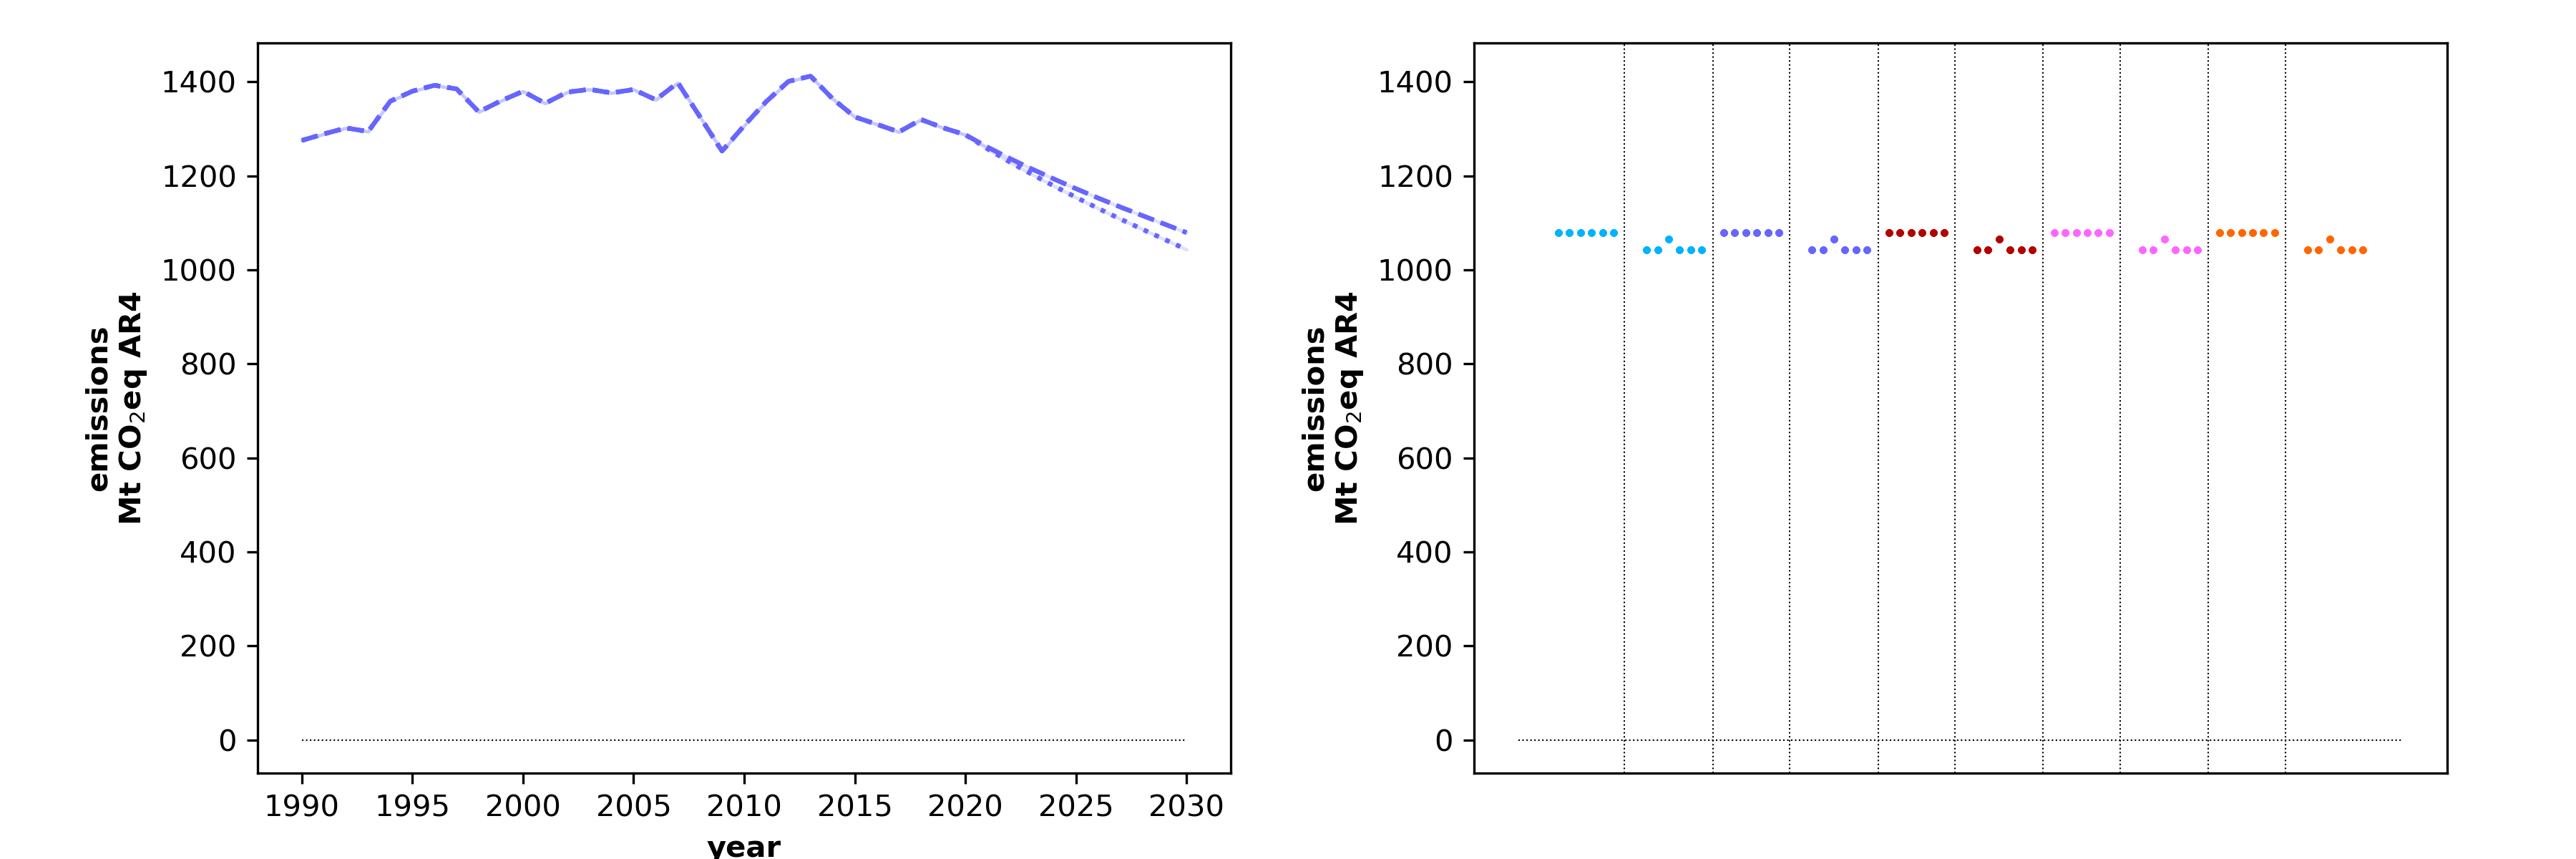
\includegraphics[width=\textwidth]{C:/Users/annikag/primap/ndc_quantifications/latex_files/JPN/ts_ndcs_quantis_JPN.png}
 \caption{Quantified mitigation targets (based on different input data and calculation options).
 Vertical lines: conditionality~/ range;
 colour coded: dmSSP1--5;
 first~/ second set of six: prio NDCs~/ SSPs;
 set of six: coverage 100, lulucf unfccc, lulucf fao, bl uncondi, const emi, estimated coverage.}
 \label{fig:miti}
 \end{figure}

 \newpage %%%
 \section{Data sources, additional information and references}
 \label{sec:dataSourcesRefs}

 \noindent \href{https://dataservices.gfz-potsdam.de/pik/showshort.php?id=escidoc:4736895}{PRIMAP-hist v2.1}: emissions from PRIMAP-hist are data from the country reported data priority scenario (HISTCR).

 \noindent \href{https://zenodo.org/record/3638137#.X2syXouxU2w}{dmSSPs}: emissions, population and GDP data are PMSSPBIE data for the five marker scenarios.

 \begin{description}
 \item [SSPs] Shared Socio-economic Pathways.
 Narratives and challenges to mitigation and adaptation: 
 SSP1: Sustainability, Taking the Green Road (low~/ low);
 SSP2: Middle of the Road (medium~/ medium);
 SSP3: Regional Rivalry, A Rocky Road (high~/ high);
 SSP4: Inequality, A Road Divided (low~/ high); and
 SSP5: Fossil-fuelled Development, Taking the Highway (high~/ low).
 \item [GDP] Gross Domestic Product. 
 Throughout this document the GDP is given as GDP~PPP, with PPP being the Purchasing Power Parity.
 \item [GWP] Global Warming Potential. we use GWP values from the IPCC 4$^{th}$ Assessment Report (AR4). 
 They reflect the forcing potential of one kilogram of a gas' emissions in comparison to one kilogram of CO$_2$ (GWP$_{CO2}$ = 1). 
 The GWPs correspond to a 100-yr period and are for CH$_4$:~25, for N$_2$O:~298, for SF$_6$:~22800, and for NF$_3$:~17200. 
 For the basket of HFC-gases the GWPs from AR4 are in the range 4--14800, and for PFCs 7190--12200. 
 To assess emissions of several GHGs, their emissions are weighted by their respective GWPs and presented in CO$_2$ equivalents (CO$_2$eq).
 \item [LULUCF] Land Use, Land-Use Change and Forestry. 
 Emissions from LULUCF are excluded throughout the document, unless stated otherwise.
 \item [Bunkers fuels] Emissions from international aviation and shipping.
 \item [Kyoto~GHG] Kyoto~GHG (Greenhouse Gas) basket: carbon dioxide (CO$_2$), methane (CH$_4$), nitrous oxide (N$_2$O), hydrofluorocarbons (HFCs), perfluorocarbons (PFCs), sulfur hexafluoride (SF$_6$), and nitrogen trifluoride (NF$_3$).
 \item [F-gases] Fluorinated gases.Basket of HFCs, PFCs, and the gases SF$_6$ and NF$_3$. 
 Some F-gases have very long atmospheric lifetimes and high Global Warming Potentials.
 \item [Target reclassification] When a country has, e.g., an RBU target (relative reduction compared to Business-As-Usual), and the BAU emissions are provided, it can be quantified based on the given emissions, and is reclassified from type\_main~RBU to type\_reclass~ABS (absolute emissions target).
 Additionally, 'NGT' targets can be reclassified as 'ABU' (absolute reduction compared to Business-As-Usual) if absolute mitigation effects due to planned policies and measures are provided.
 \end{description}

 \noindent \textbf{Links to additional information:}
 \begin{itemize}
 \item \href{https://www.climatewatchdata.org/}{CLIMATEWATCH} 
 \vspace{-.2cm} \item \href{https://www.carbonbrief.org/}{CarbonBrief: Clear on Climate} 
 \vspace{-.2cm} \item \href{https://climateactiontracker.org/}{Climate Action Tracker} 
 \vspace{-.2cm} \item \href{https://zenodo.org/record/3638137#.X2sqPIuxU2w}{Country resolved combined emission and socio-economic pathways based on the RCP and SSP scenarios} (February 2020)
 \vspace{-.2cm} \item \href{https://www.carbonbrief.org/guest-post-calculating-the-true-climate-impact-of-aviation-emissions?utm_campaign=Carbon%20Brief%20Daily%20Briefing&utm_medium=email&utm_source=Revue%20newsletter}{Guest post: Calculating the true climate impact of aviation emissions} (September 2020)
 \vspace{-.2cm} \item \href{https://www.iges.or.jp/en/pub/iges-indc-ndc-database/en}{IGES NDC Database} 
 \vspace{-.2cm} \item \href{https://www.ipcc.ch/}{IPCC (The Intergovernmental Panel on Climate Change)} 
 \vspace{-.2cm} \item \href{https://www.ipcc.ch/sr15/}{IPCC Special Report: Global Warming of 1.5$^{\circ}$} (2018)
 \vspace{-.2cm} \item \href{https://www.isimip.org/isipedia/#isipedia-portal}{ISIMIP~/ ISIpedia} 
 \vspace{-.2cm} \item \href{https://klimalog.die-gdi.de/ndc/#NDCExplorer/worldMap?NDC??income???catIncome}{NDC Explorer} 
 \vspace{-.2cm} \item \href{https://ndcpartnership.org/}{NDC PARTNERSHIP} 
 \vspace{-.2cm} \item \href{https://themasites.pbl.nl/o/climate-ndc-policies-tool/}{PBL Climate Pledge NDC tool} 
 \vspace{-.2cm} \item \href{https://tntcat.iiasa.ac.at/SspDb/dsd?Action=htmlpage&page=about}{SSP Database (Shared Socioeconomic Pathways) - Version 2.0} (December 2018)
 \vspace{-.2cm} \item \href{https://dataservices.gfz-potsdam.de/pik/showshort.php?id=escidoc:4736895}{The PRIMAP-hist national historical emissions time series (1850-2017)} (2019)
 \vspace{-.2cm} \item \href{https://unfccc.int/}{UNFCCC (United Nations Framework Convention on Climate Change)} 
 \vspace{-.2cm} \item \href{https://www.theguardian.com/environment/2020/sep/21/worlds-richest-1-cause-double-co2-emissions-of-poorest-50-says-oxfam?utm_campaign=Carbon%20Brief%20Daily%20Briefing&utm_medium=email&utm_source=Revue%20newsletter}{World's richest 1\% cause double CO$_2$ emissions of poorest 50\%, says Oxfam} 
 \vspace{-.2cm} \item \href{https://www.showyourbudgets.org/de/?country=whole_world}{\#showyourbudgets} 
 \end{itemize}

 %%%
 \end{document}
